\chapter{Apéndice}
%\lstinputlisting[language=bash,basicstyle=\ttfamily\scriptsize,caption={Archivo de ingesta de Sifode Calificación}]{code/sifode_calificacion.sh}
%\pagebreak
%\lstinputlisting[language=bash,basicstyle=\ttfamily\scriptsize,caption={Archivo de ingesta de Sifode Domicilio}]{code/sifode_domicilio.sh}
%\pagebreak
%\lstinputlisting[language=python,basicstyle=\ttfamily\scriptsize,caption={Archivo de ingesta de Sifode}]{code/sifode.py}
%\pagebreak
%\lstinputlisting[language=json,basicstyle=\ttfamily\scriptsize,caption={Catálogo},breaklines=true]{code/catalog.json}
\section{Estructuras ajustadas de cada modelo}
\begin{figure}
    \caption{Modelo sin restricciones}
    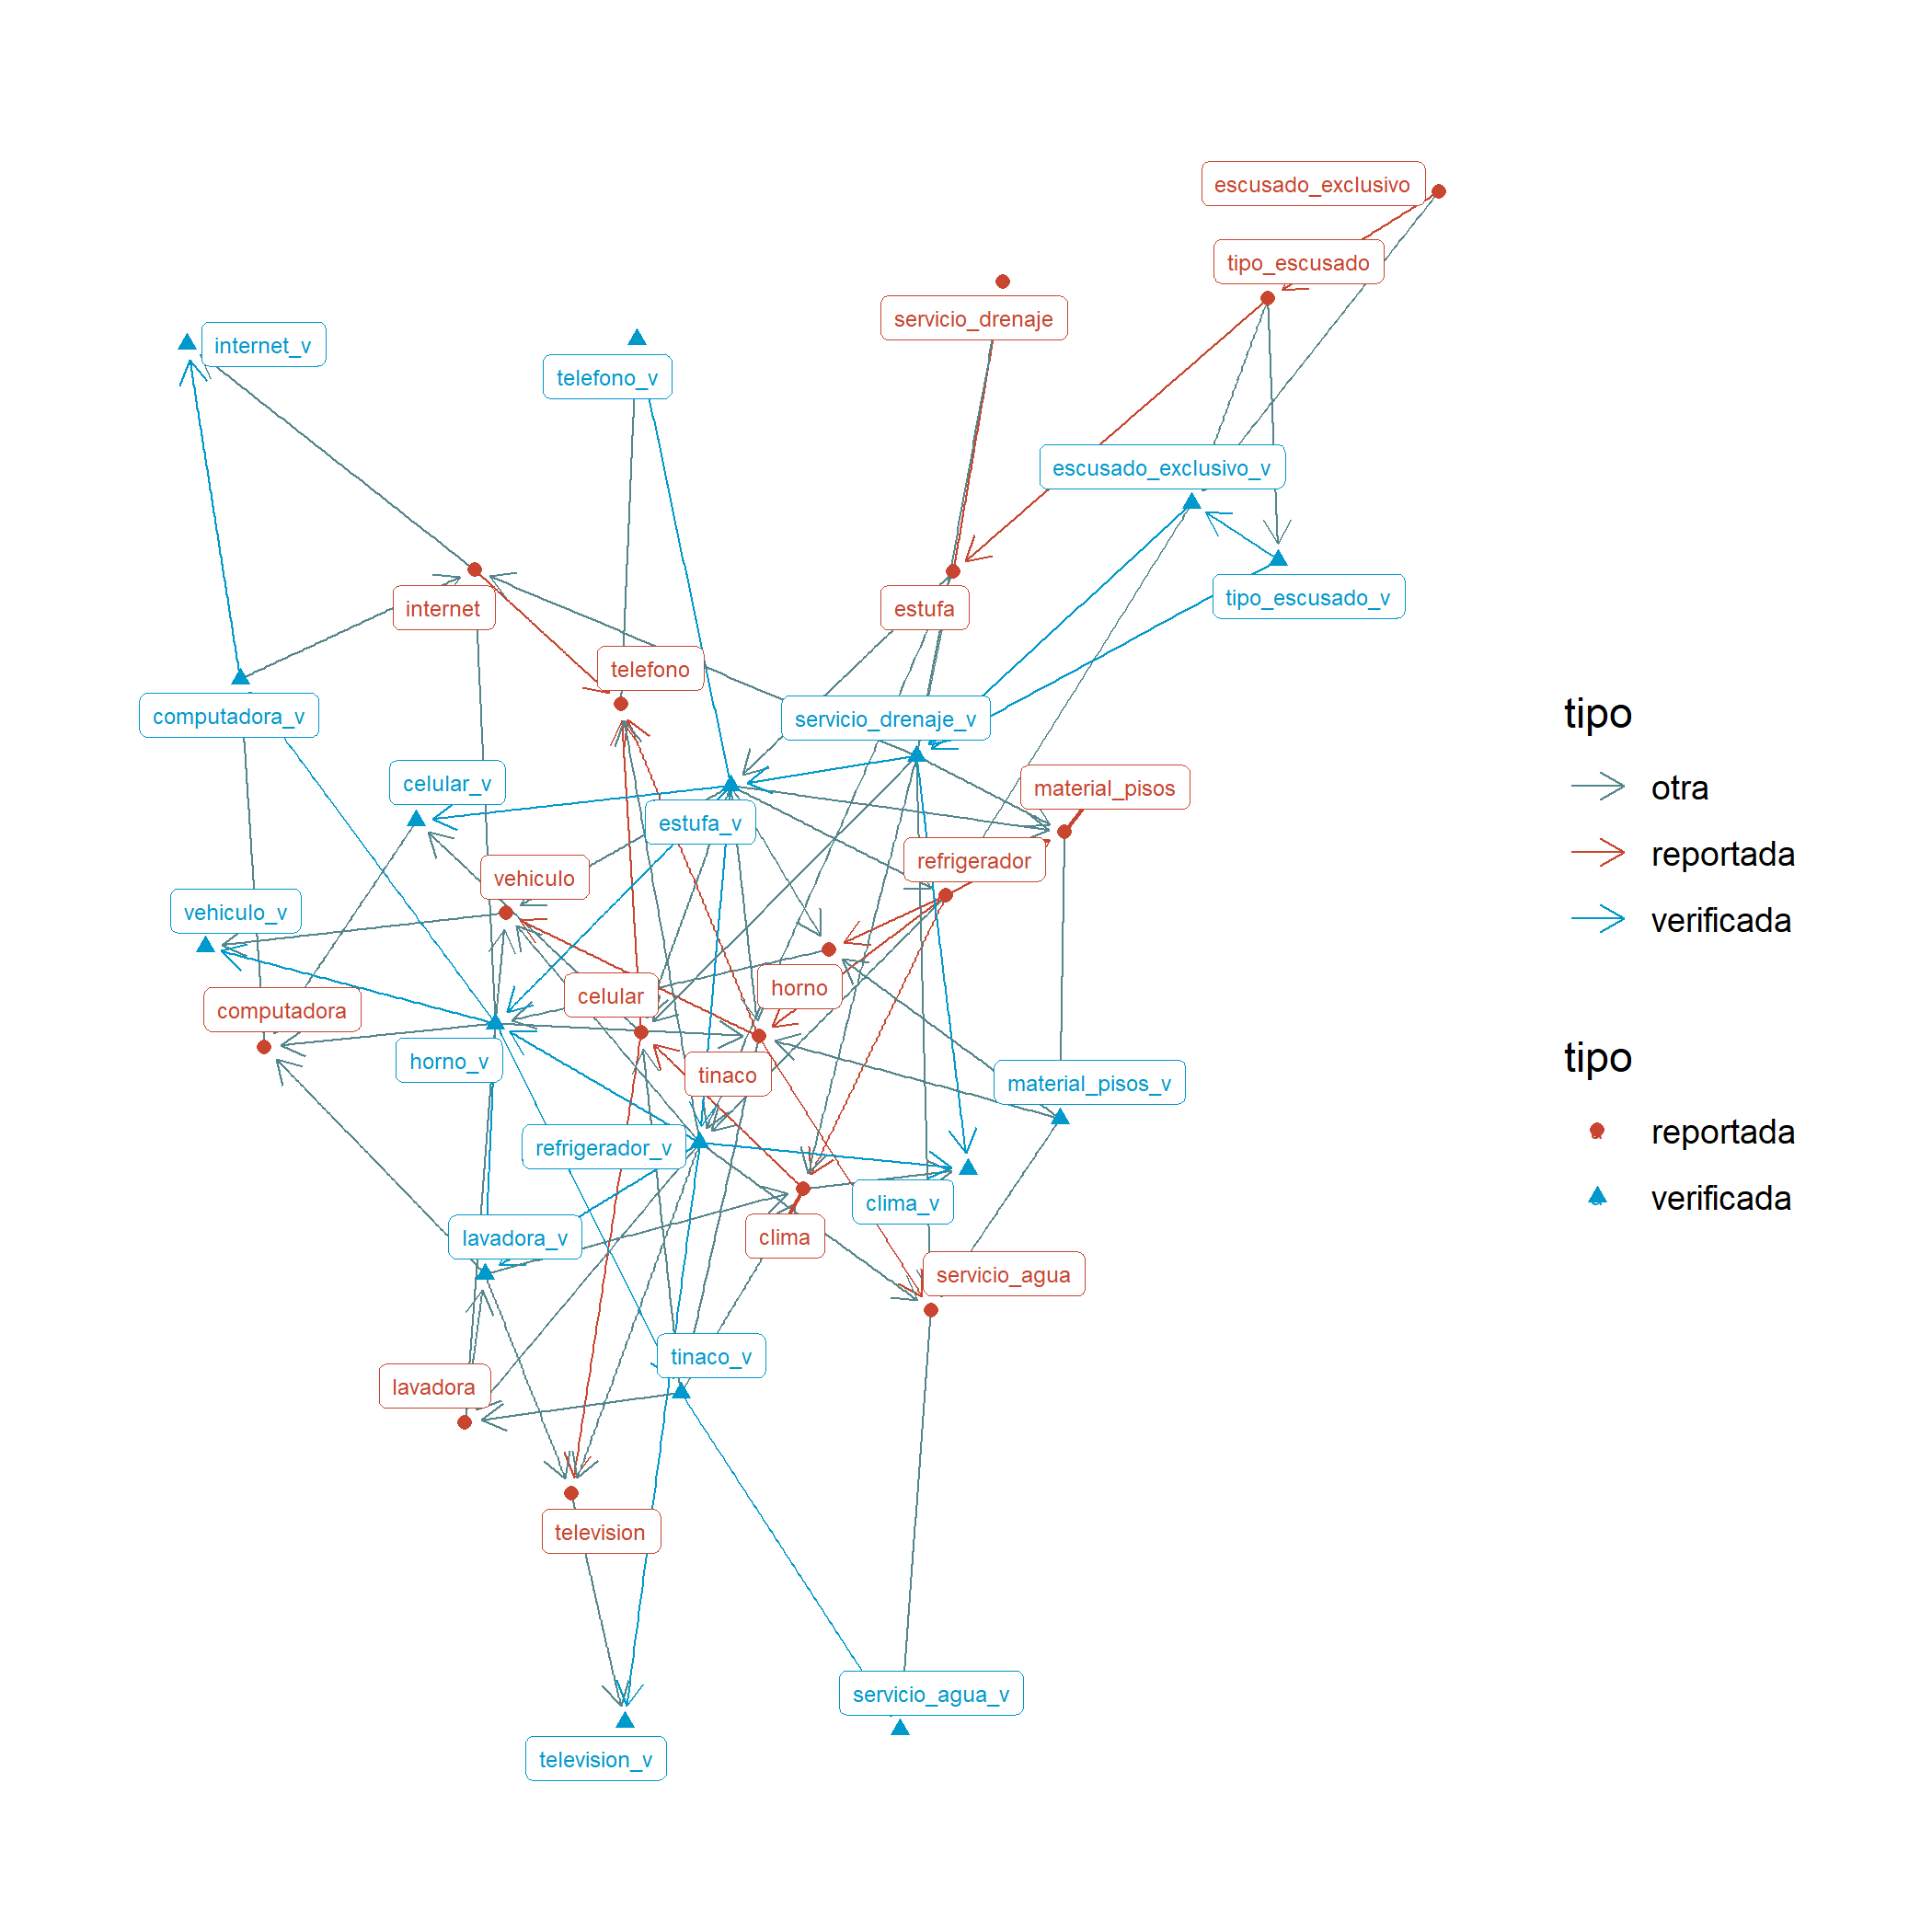
\includegraphics[width=18cm, height=18cm]{p_dag}
\end{figure}
\pagebreak
\begin{figure}
    \caption{Modelo base + variables municipales + grado de marginación}
    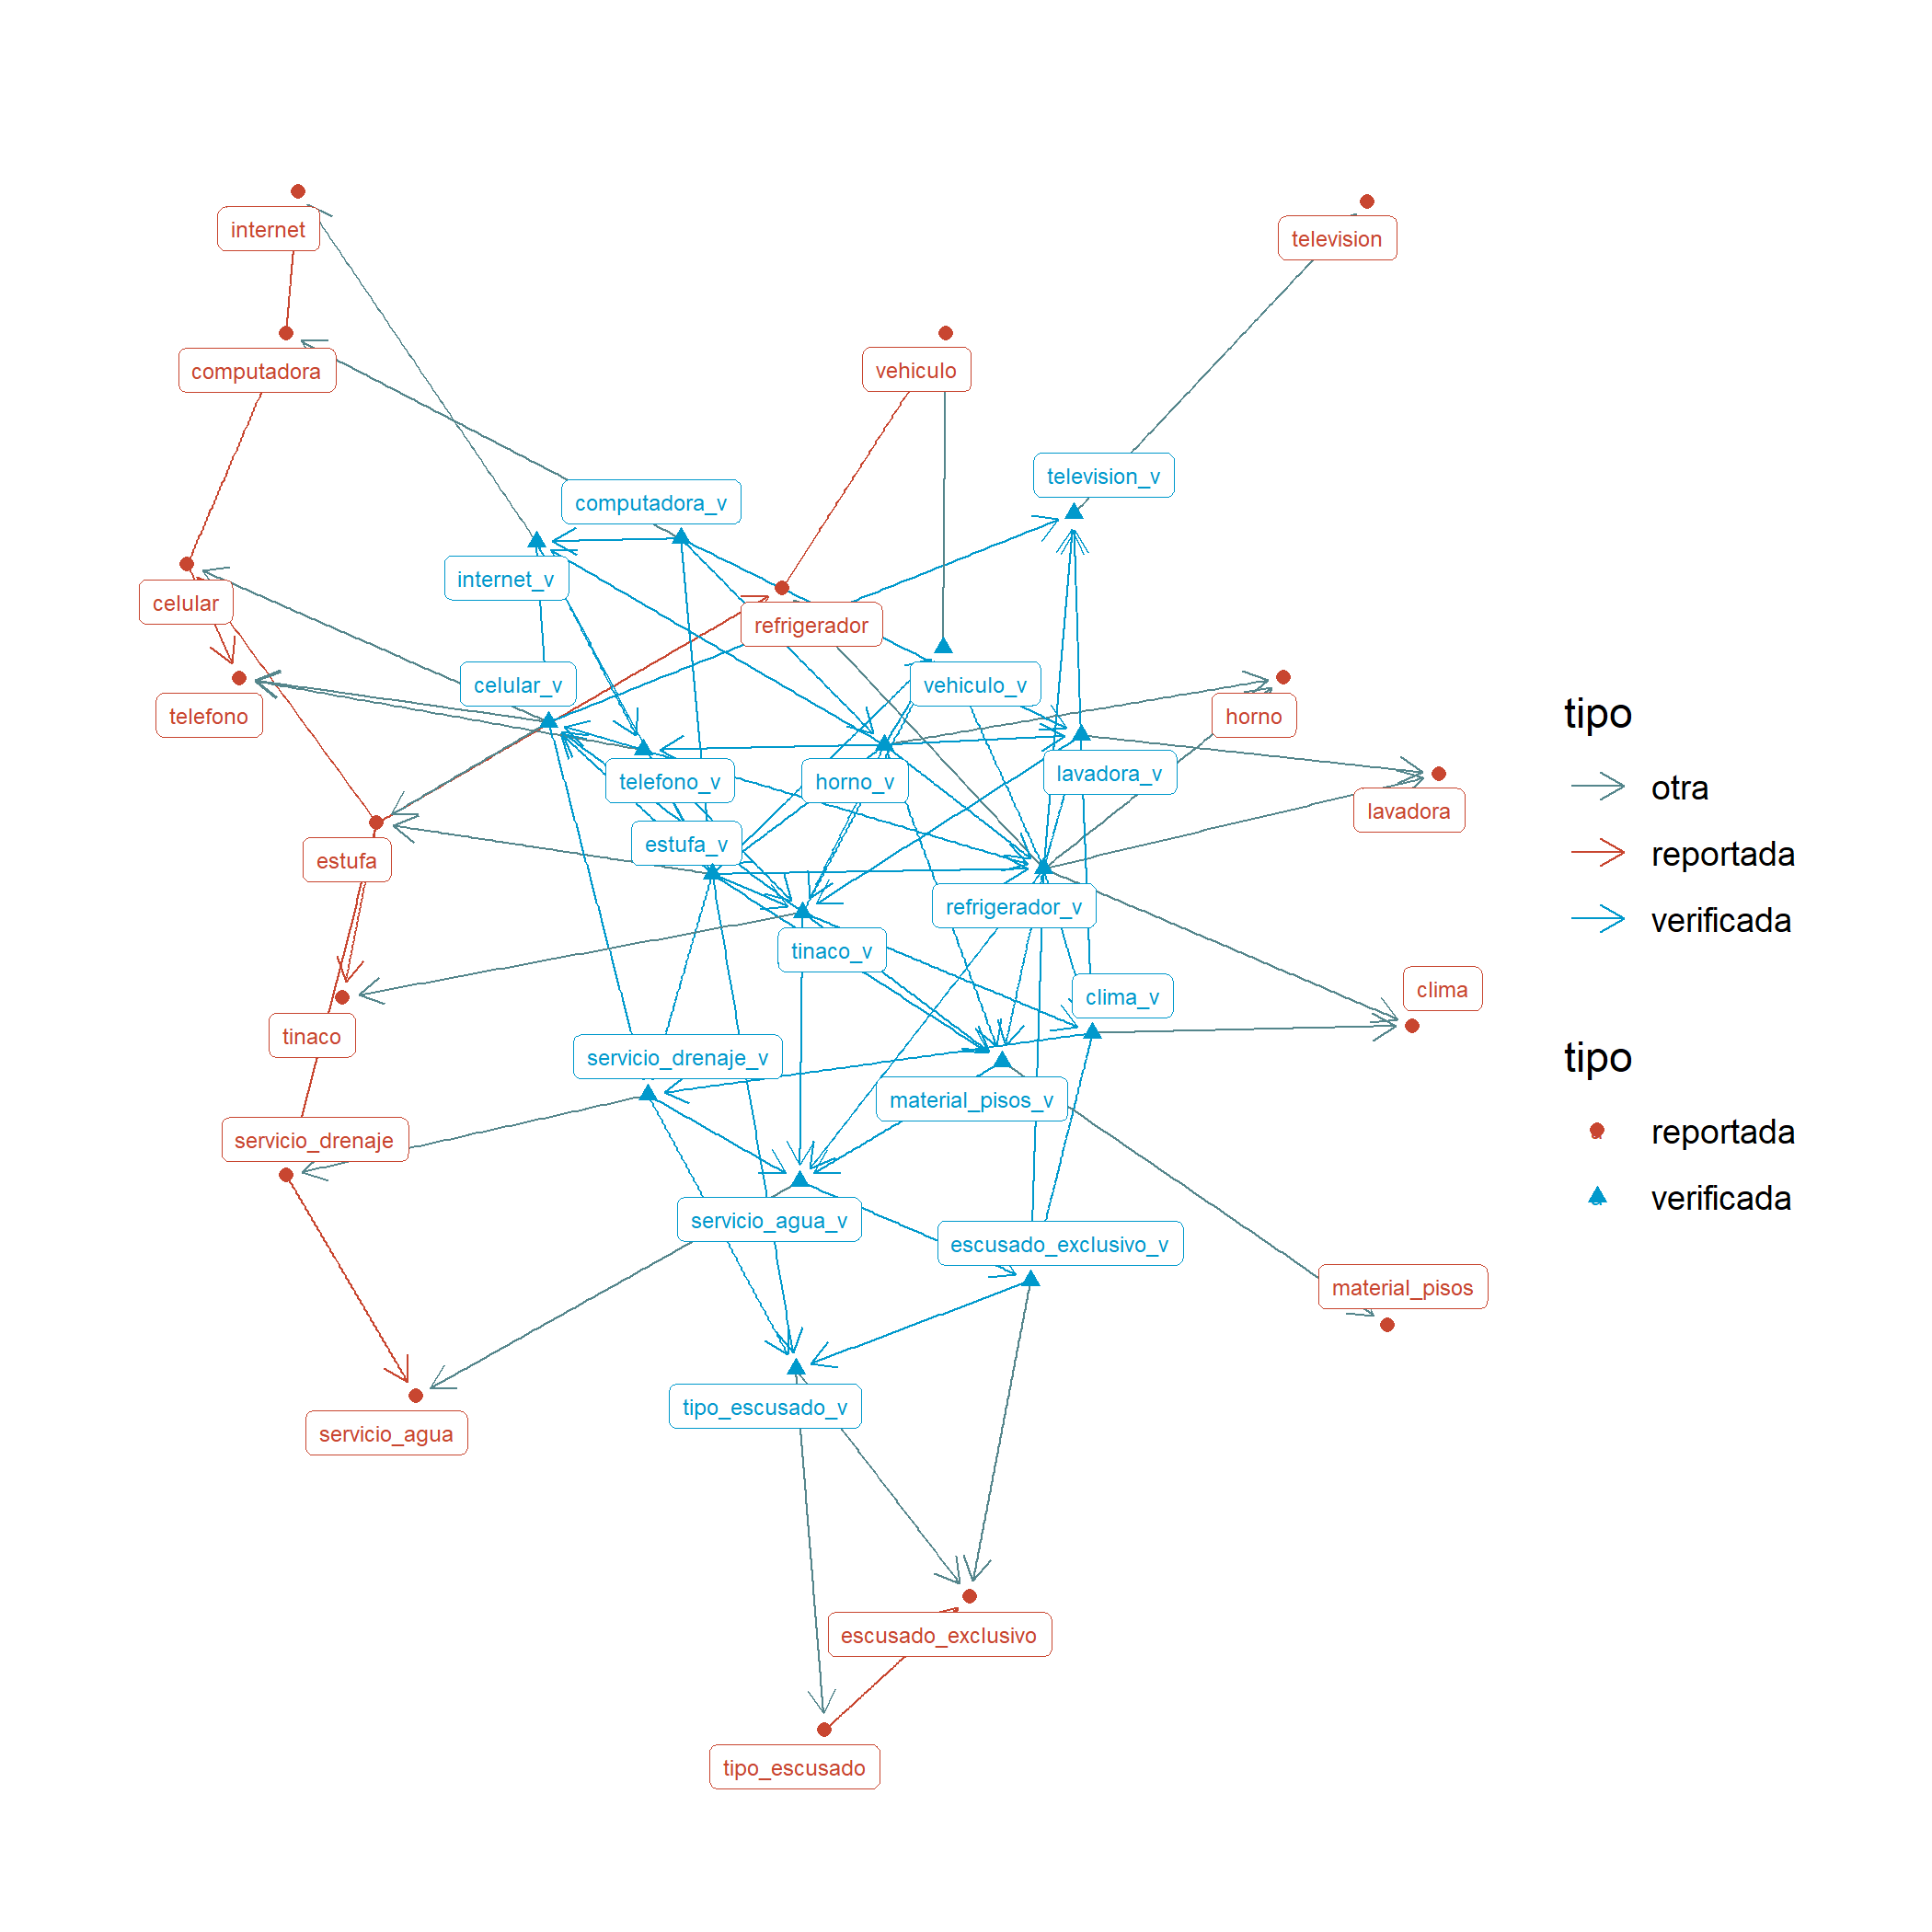
\includegraphics[width=18cm, height=18cm]{p_dag_1}
\end{figure}
\pagebreak
\begin{figure}
    \caption{Modelo base + grado de marginación}
    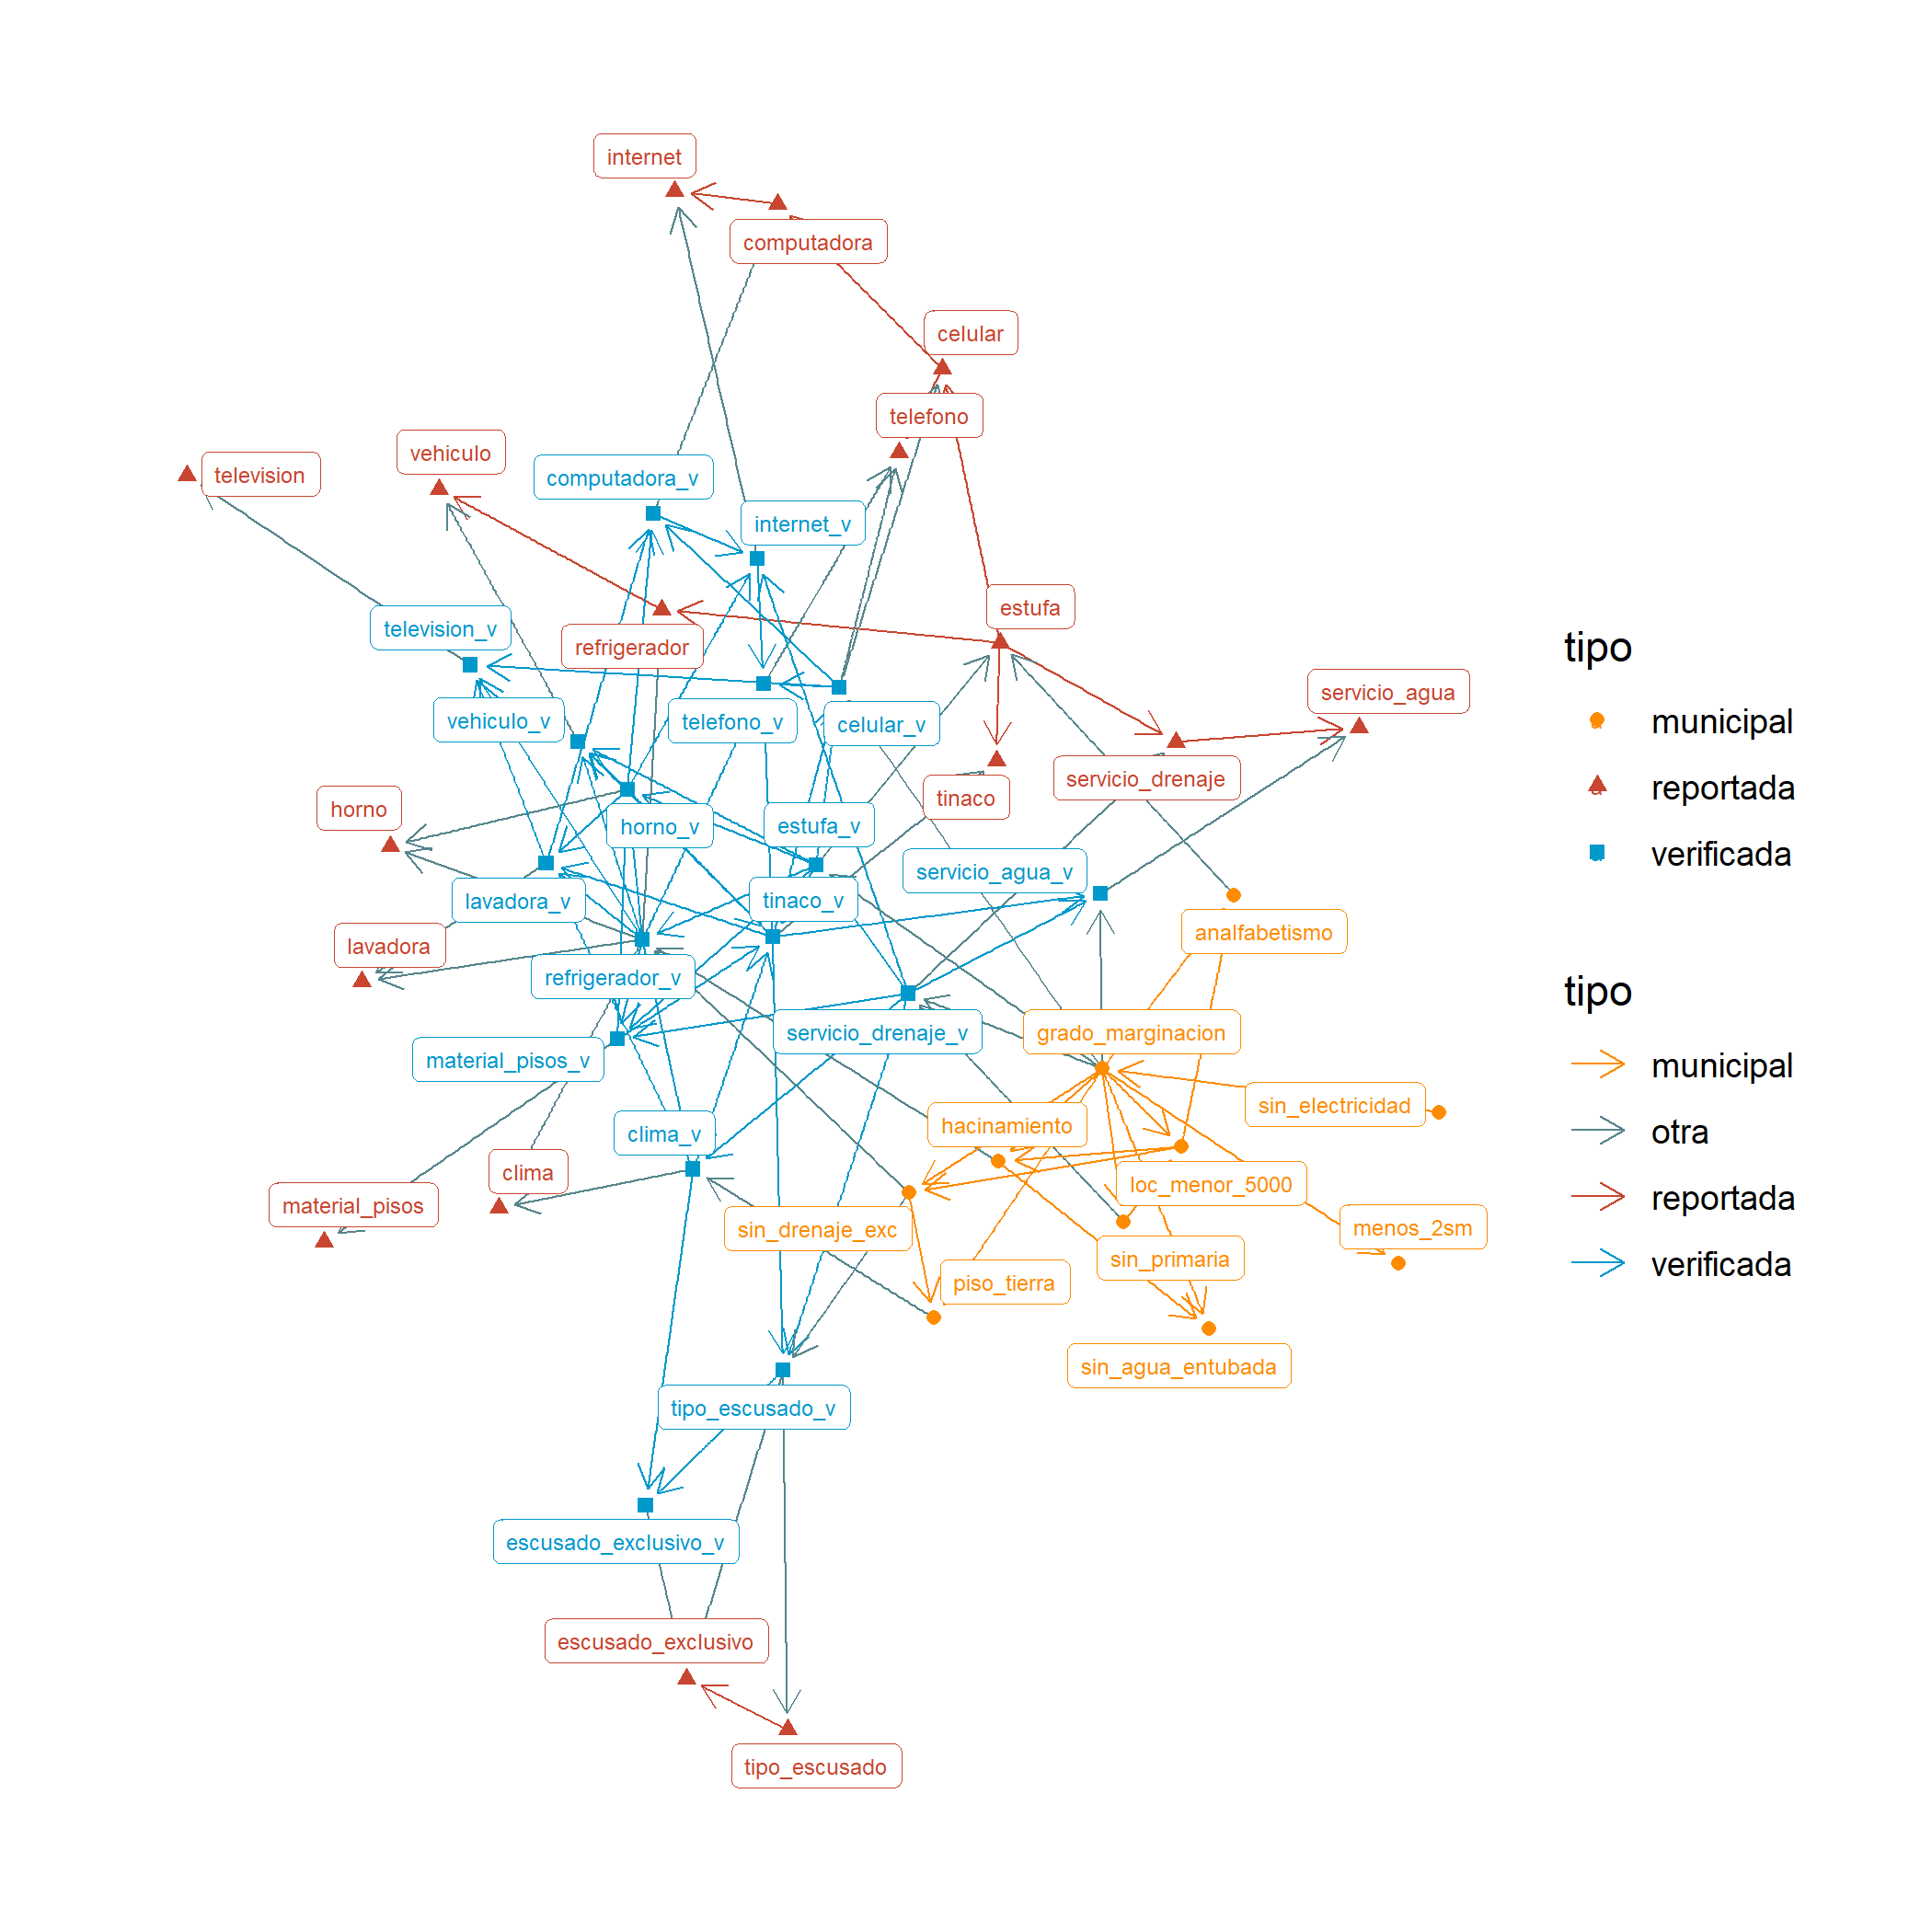
\includegraphics[width=18cm, height=18cm]{p_dag_mun1}
\end{figure}
\pagebreak
\begin{figure}
    \caption{Modelo base + variables municipales}
    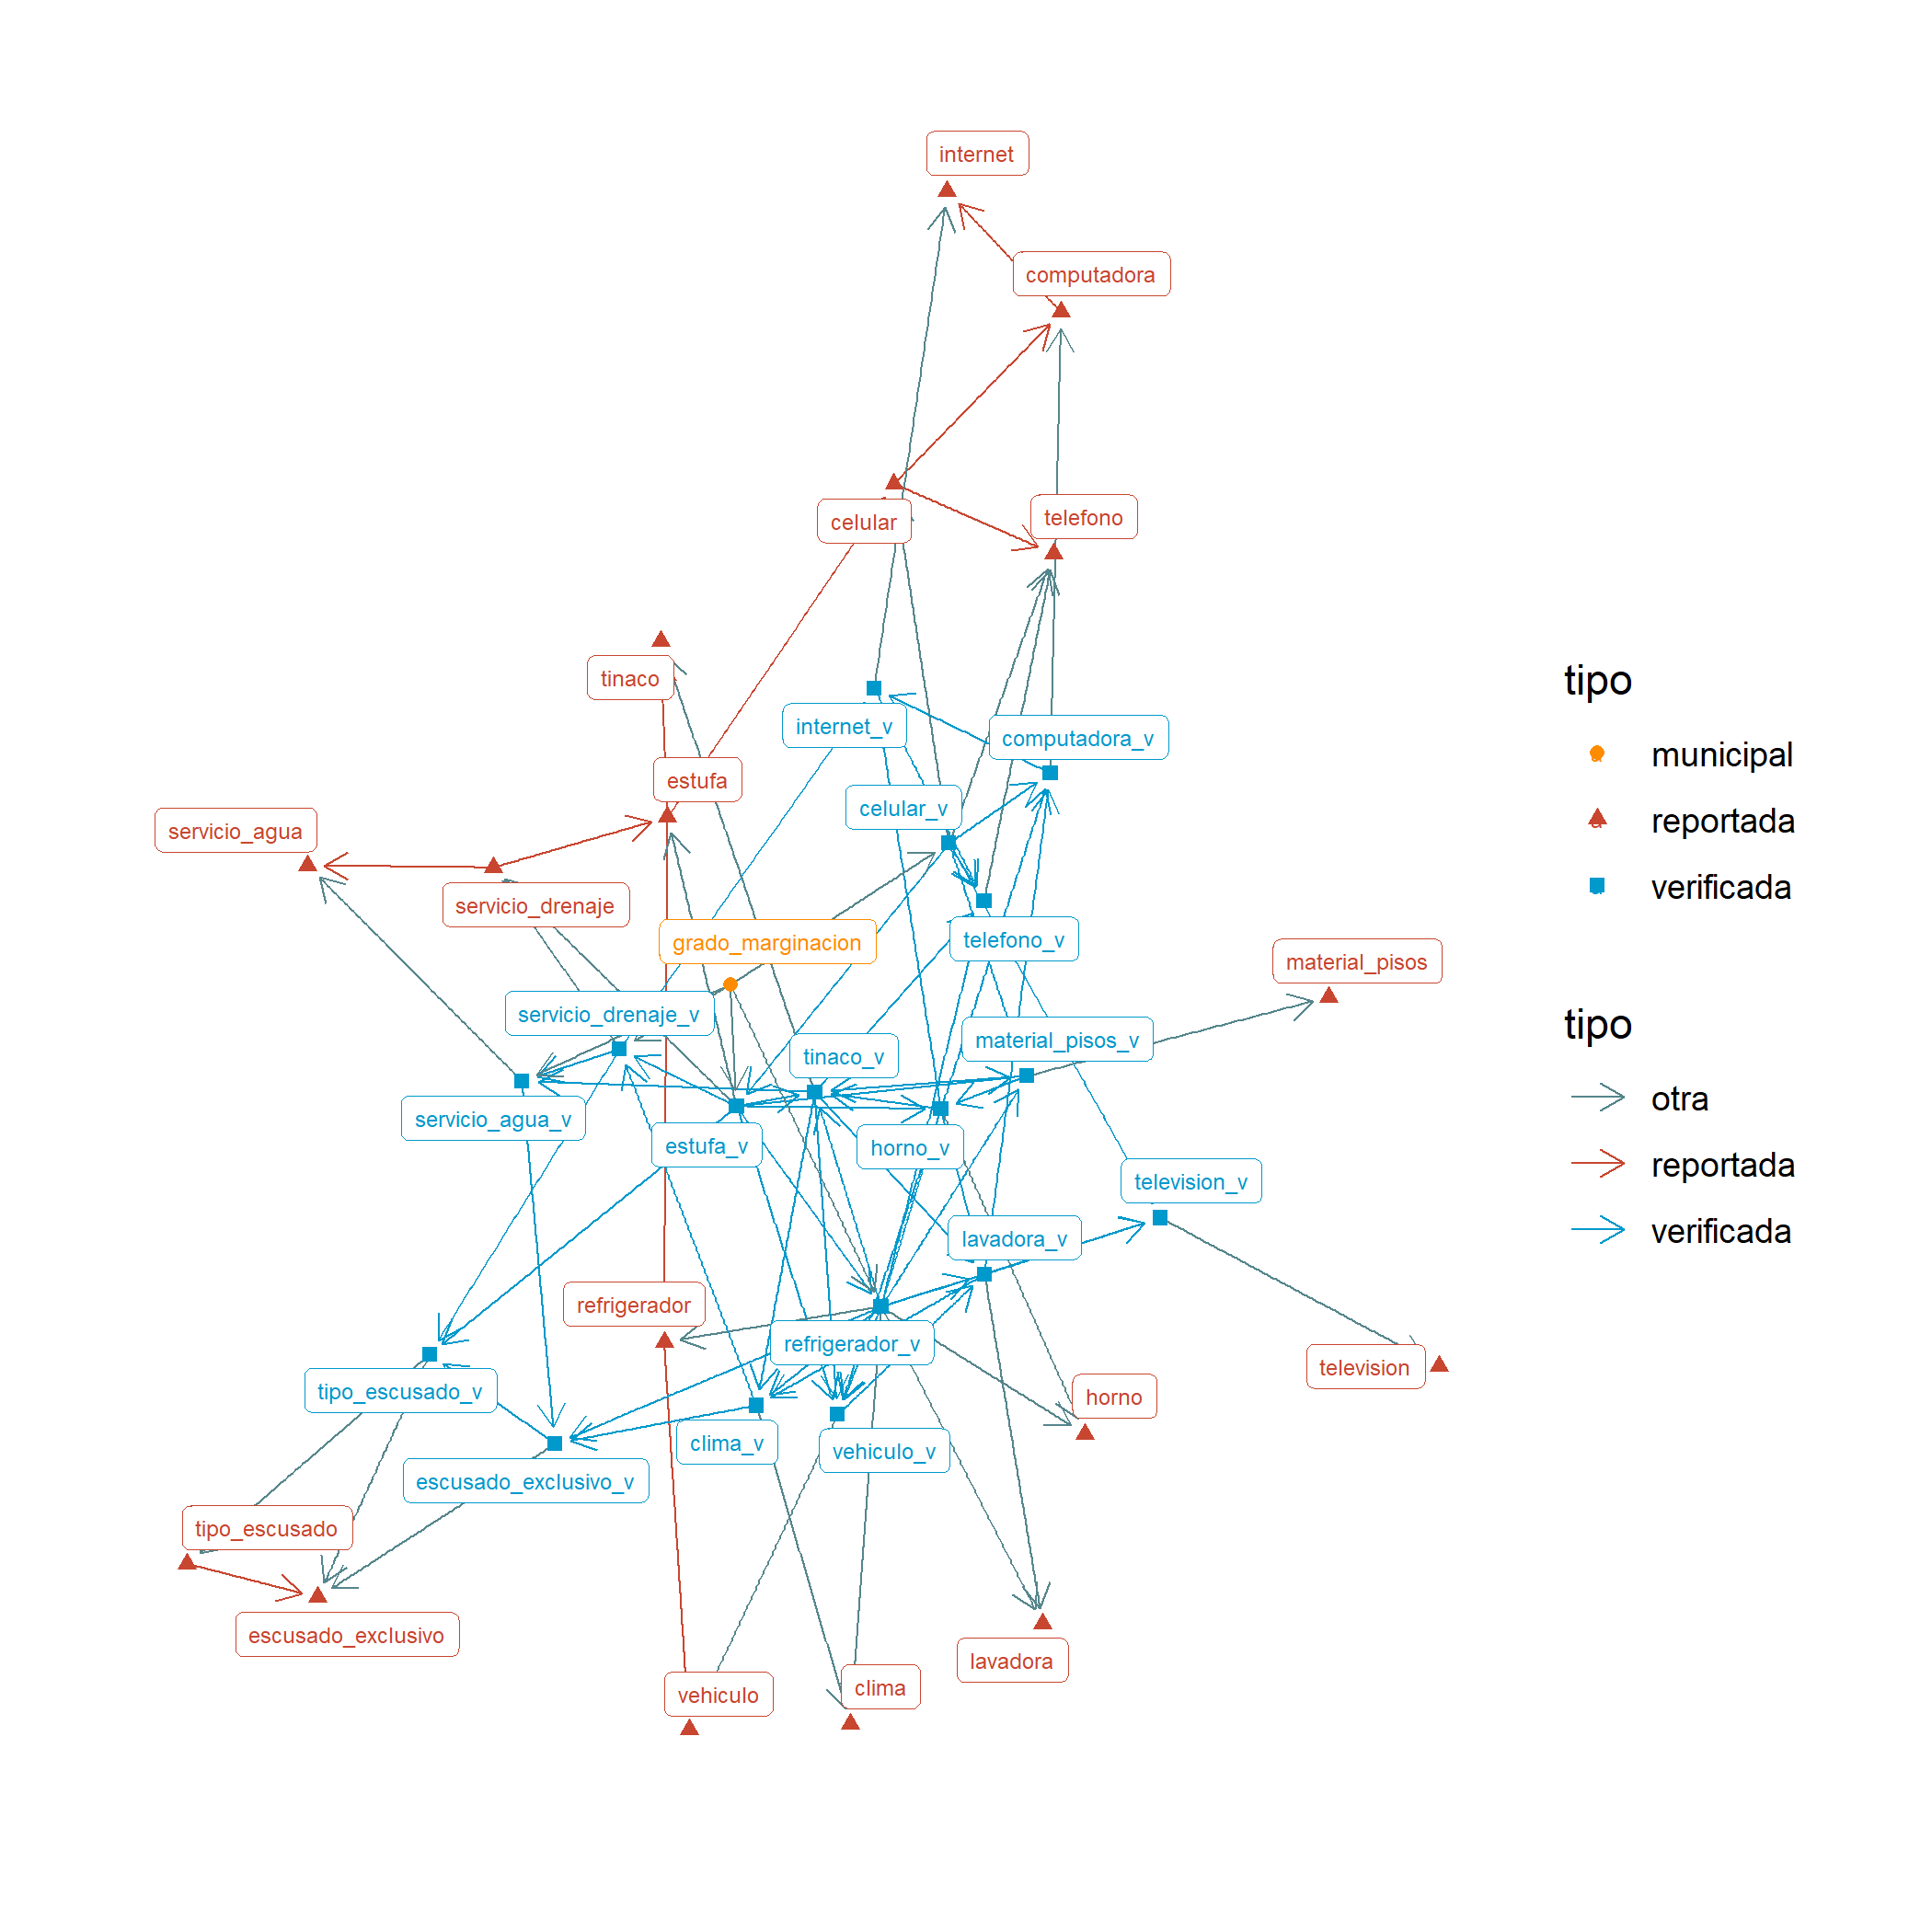
\includegraphics[width=18cm, height=18cm]{p_dag_mun2}
\end{figure}
\pagebreak
\begin{figure}
    \caption{Modelo base + 3 variables municipales}
    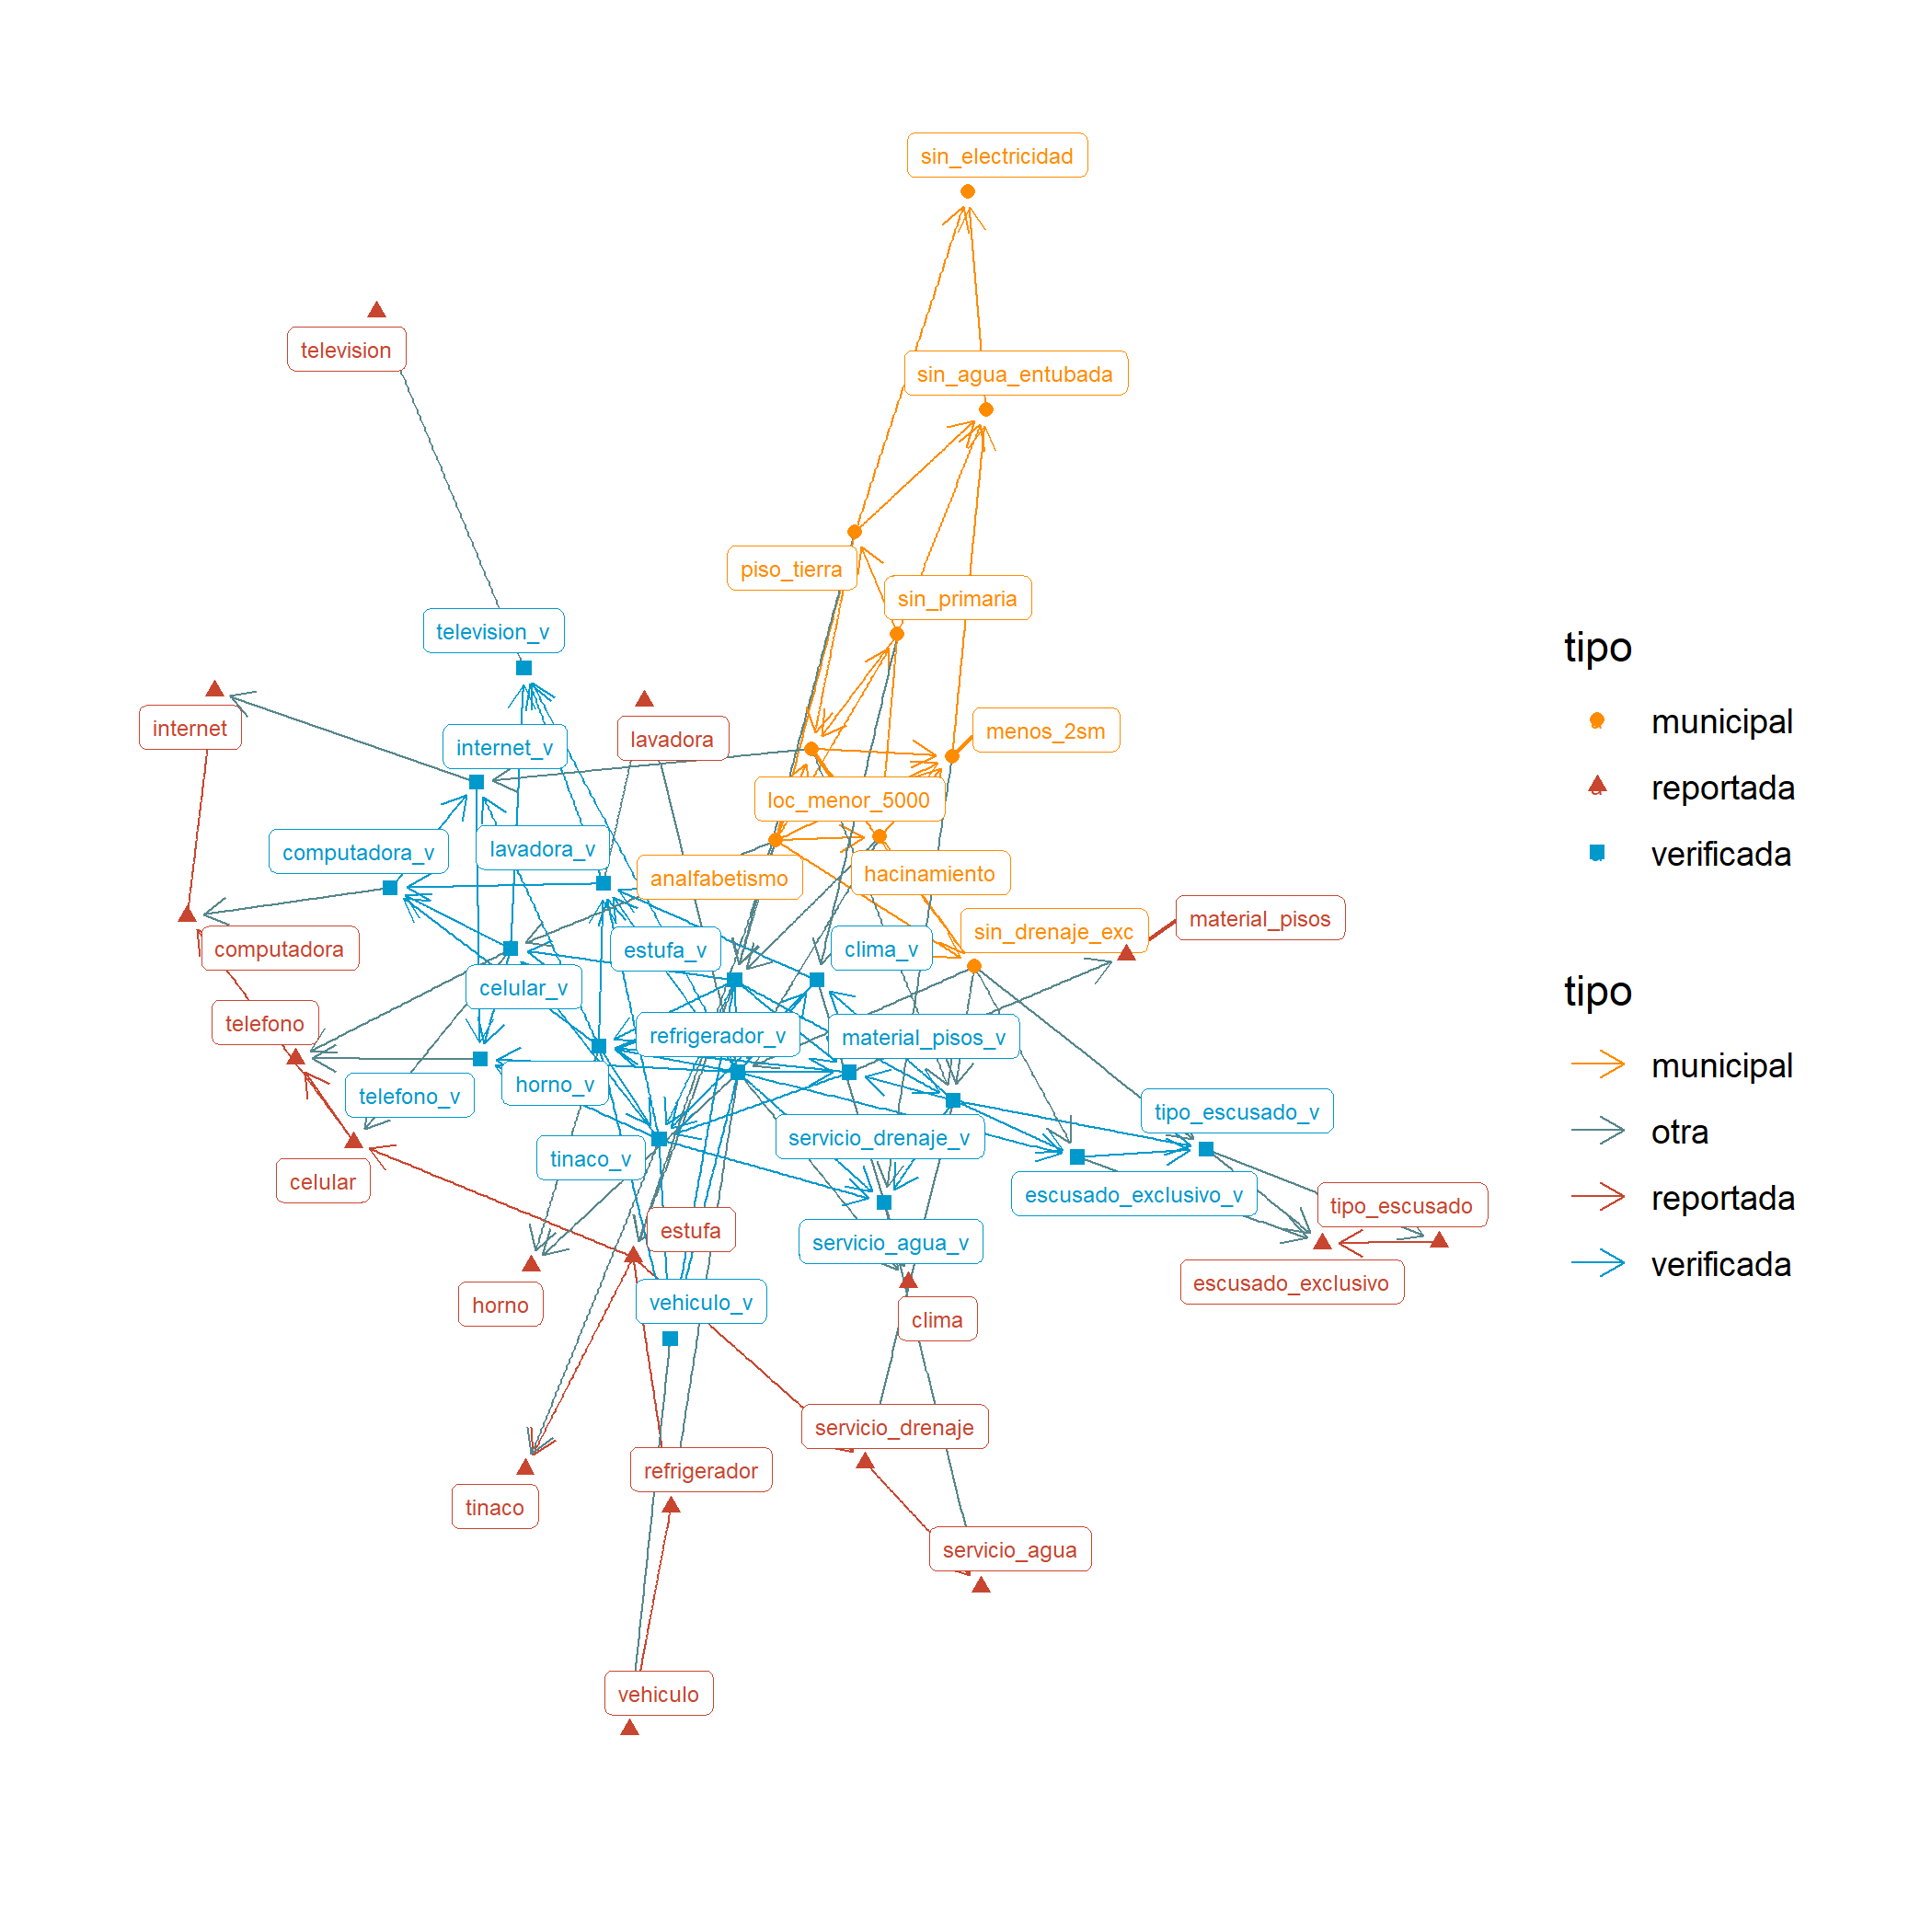
\includegraphics[width=18cm, height=18cm]{p_dag_mun3}
\end{figure}
\pagebreak
\section{Código}
\lstinputlisting[language=R,basicstyle=\ttfamily\scriptsize,caption={Funciones auxiliares para el ajuste e inferencia en Redes Bayesianas}]{code/graph_models_funs.R}
\pagebreak
\lstinputlisting[language=R,basicstyle=\ttfamily\scriptsize,caption={Código de exploración, análisis y ajuste del modelo}]{code/exploracion.R}
